\documentclass{article}
% \documentclass[draft]{article}


% ----------------Report particulars --------------------%
\title{Remote Sensing Notes} 
\author{Rosa Trancoso}
% \date{\today\\v0.1}
\date{\filemodprint{report.tex}\\v0.1}


% Usual latex stuff
%----------- Load user packages (optional) --------------%

\usepackage{filemod}
% Language and font encodings
\usepackage[english]{babel}
\usepackage[utf8x]{inputenc}
\usepackage[T1]{fontenc}

% \usepackage[scaled]{uarial}
% \renewcommand{\familydefault}{\sfdefault}

% Sets page size and margins
\usepackage{parskip}

\usepackage{amsmath}
\usepackage[pdftex]{graphicx}

\usepackage{acro}  % printacronyms

\usepackage[a4paper]{geometry} % textwidth 418pt (14cm) instead of 345pt (12...cm)

% % other
% \usepackage[colorinlistoftodos]{todonotes}
\usepackage[colorlinks=true, allcolors=blue]{hyperref}
\usepackage{soul} % hl

\usepackage[font={small},figurewithin={section}]{caption}
% \usepackage{natbib}
\usepackage{url}
\usepackage{booktabs} % toprule
\usepackage{tabularx}
\newcolumntype{L}[1]{>{\hsize=#1\hsize\raggedright\arraybackslash}X}%
\newcolumntype{R}[1]{>{\hsize=#1\hsize\raggedleft\arraybackslash}X}%
\newcolumntype{C}[1]{>{\hsize=#1\hsize\centering\arraybackslash}X}%

\makeatletter
 \renewenvironment{table}
     {\@float{table} \small}
     {\end@float}
 \makeatother


% \usepackage{tabto}
% \usepackage[]{dirtree}
% \usepackage{multimedia}
% \usepackage{pdfpages}
\usepackage{longtable}

\usepackage{xspace}

\usepackage{layouts} % \printinunitsof{cm}\prntlen{\textwidth}

\usepackage[section]{placeins}  % Dump floats before next section


\usepackage{titlesec}  % make paragraph have numbers
\setcounter{secnumdepth}{5}
\setcounter{tocdepth}{5}

% new line after paragraph

\titleformat{\paragraph}
{\normalfont\normalsize\bfseries}{\theparagraph}{1em}{}
\titlespacing*{\paragraph}
{0pt}{3.25ex plus 1ex minus .2ex}{1.5ex plus .2ex}




%-------------- Definitions (optional) -----------------%

\def\deg{$^\circ$\xspace}
\def\ms{m s\textsuperscript{-1}\xspace}

\DeclareAcronym{ec}{short=EC,long=European Commission} 
\DeclareAcronym{esa}{short=ESA,long=European Space Agency}
\DeclareAcronym{geoss}{short=GEOSS,long=Global Earth Observation System of Systems}
\DeclareAcronym{gmes}{short=GMES,long=Global Monitoring for Environment and Security programme}
\DeclareAcronym{isar}{short=ISAR,long=Inverse Synthetic Aperture Radar}
\DeclareAcronym{miras}{short=MIRAS,long=Microwave Imaging Radiometer using Aperture Synthesis}
\DeclareAcronym{mtg}{short=MTG,long=Meteosat Third Generation}
\DeclareAcronym{mtg-s}{short=MTG-S,long=Meteosat Third Generation-Sounder}
\DeclareAcronym{sar}{short=SAR,long=Synthetic Aperture Radar}
\DeclareAcronym{smos}{short=SMOS,long=Soil Moisture Ocean Salinity}

\DeclareAcronym{agri}{short=AGRI,long=Advanced Geosynchronous Radiation Imager}
\DeclareAcronym{fd}{short=FD,long=Full Disk}
\DeclareAcronym{vissr}{short=VISSR,long=Visible and Infrared Spin-Scan Radiometer}
\DeclareAcronym{giirs}{short=GIIRS,long=Geostationary Interferometric Infrared Sounder}
\DeclareAcronym{lmi}{short=LMI,long=Ligthning Mapping Imager}
\DeclareAcronym{sep}{short=SEP,long=Space Environment Package}
\DeclareAcronym{sem}{short=SEM,long=Space Environment Monitor}
\DeclareAcronym{cma}{short=CMA,long=China Meteorological Administration}
\DeclareAcronym{cast}{short=CAST,long=China Academy of Space Technology}


% \DeclareAcronym{cfsr}{short=CFSR,long=Climate Forecast System Reanalysis}
% \DeclareAcronym{ncep}{short=NCEP,long=National Centers for Enviromental Prediction}
% \DeclareAcronym{nhc}{short=NHC,long=National Hurricane Center}
% \DeclareAcronym{sst}{short=SST,long=Sea Surface Temperature}
% \DeclareAcronym{st2}{short=ST2,long=\citet{short=,long=short=hereafter ST2,long=Tolman:1996}}


% --------------- Beginning Document --------------------%
\begin{document}
\maketitle

\begin{abstract}
the abstract should have 6 sentences. 1. Topic 2. Importance 3. Here we

textwidth in pt: \the\textwidth

textwidth in cm: \printinunitsof{cm}\prntlen{\textwidth}
 
\end{abstract}

\tableofcontents

% ------------------------------------------
% Introduction
% ------------------------------------------
\section{Introduction}
\label{sec:intro}


Remote sensing is the scanning of the earth by satellite or high-flying aircraft in order to obtain information about it.
Remote sensing is the acquisition of information about an object or phenomenon without making physical contact with the object and thus in contrast to on-site observation\footnote{\url{https://en.wikipedia.org/wiki/Remote_sensing}}.

Remote sensors can be either passive or active. \textbf{Passive} sensors respond to external stimuli. They record natural energy that is reflected or emitted from the Earth's surface. The most common source of radiation detected by passive sensors is reflected sunlight. In contrast, \textbf{active} sensors use internal stimuli to collect data about Earth. For example, a laser-beam remote sensing system projects a laser onto the surface of Earth and measures the time that it takes for the laser to reflect back to its sensor\footnote{\url{http://oceanservice.noaa.gov/facts/remotesensing.html}}.

Examples of passive remote sensors include film photography, infrared, charge-coupled devices, and radiometers (wiki).

Examples of active remote sensors are Radar and Lidar where the time delay between emission and return is measured, establishing the location, speed and direction of an object (wiki).

The quality of remote sensing data consists of its spatial, spectral, radiometric and temporal resolutions.

\subsection{Electromagnetic Spectrum}

\begin{figure}[!ht]    
\centering
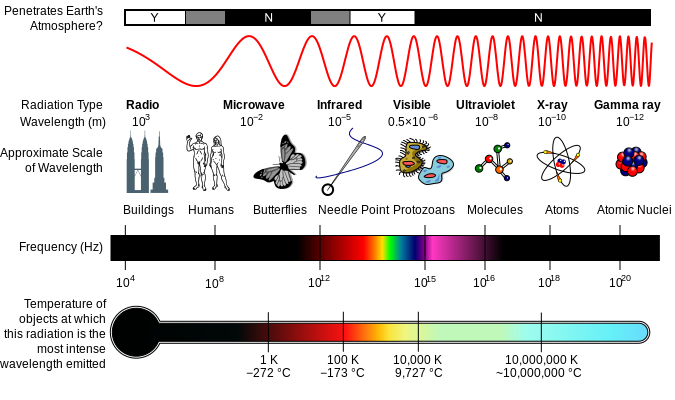
\includegraphics[width=\textwidth]{figures/EM_Spectrum_Properties_edit.png}
\caption{A diagram of the electromagnetic spectrum, showing various properties across the range of frequencies and wavelengths. Source: \url{https://en.wikipedia.org/wiki/Electromagnetic_spectrum}}
\label{fig:spectrum1}
\end{figure}

\begin{figure}[h!]    
\centering
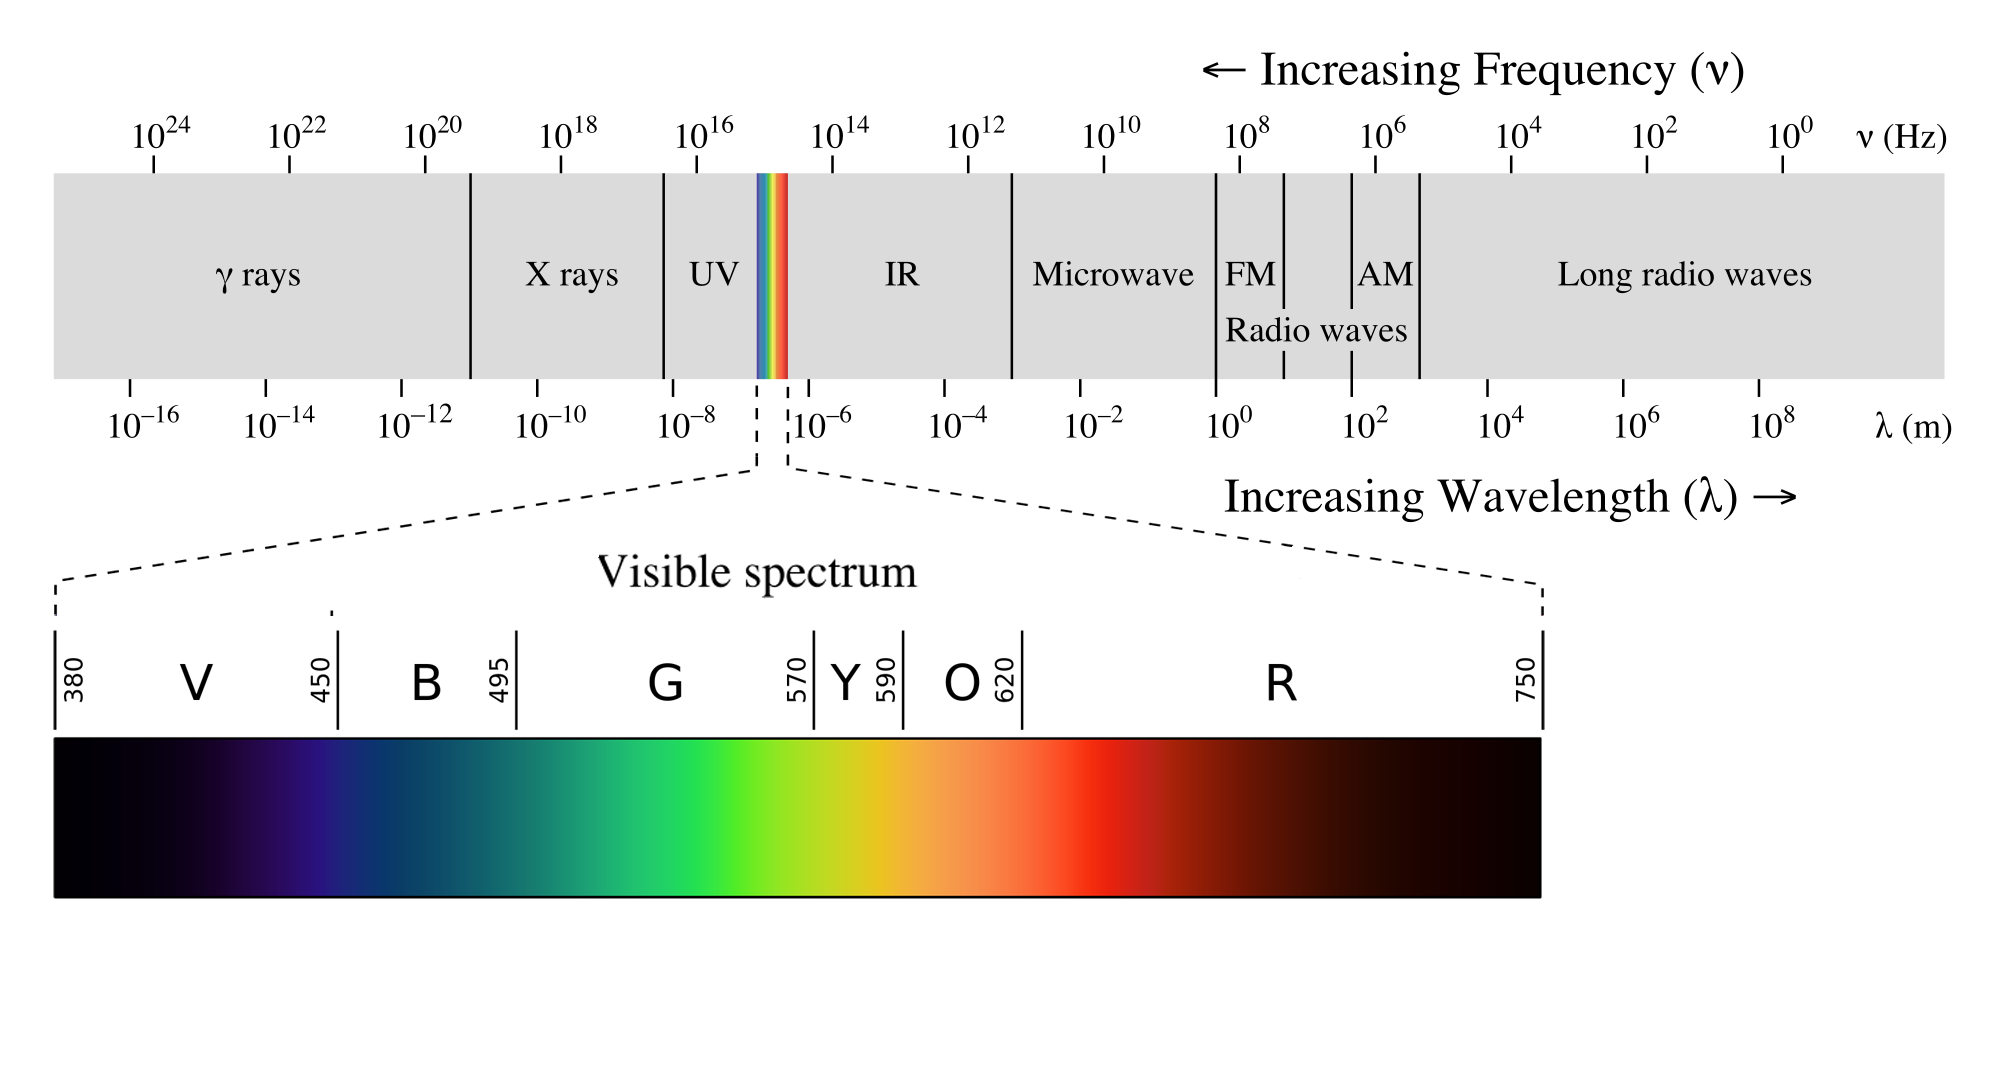
\includegraphics[width=\linewidth]{figures/EM_spectrumrevised.png}`
\caption{Electromagnetic Spectrum with Visible light highlighted. Source: \url{https://en.wikipedia.org/wiki/Electromagnetic_radiation}}
\label{fig:spectrum2}
\end{figure}


\begin{figure}[h!]    
\centering
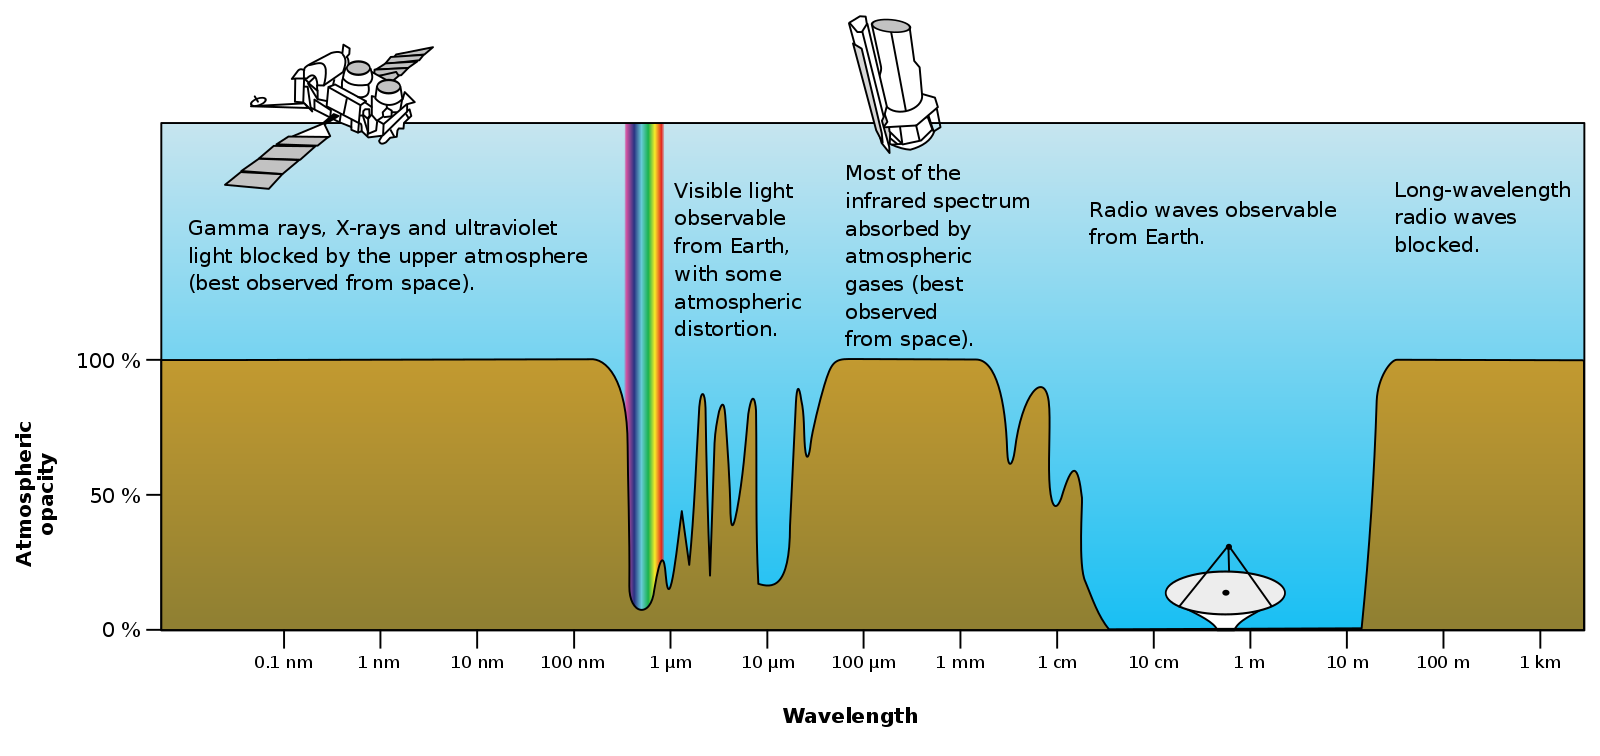
\includegraphics[width=\linewidth]{figures/Atmospheric_electromagnetic_opacity.png}
\caption{Electromagnetic transmittance, or opacity, of the Earth's atmosphere. Source: \url{https://en.wikipedia.org/wiki/Electromagnetic_radiation}}
\label{fig:atm_opacity}
\end{figure}

\subsection{Radar}
Radar is an object-detection system that uses radio waves to determine the range, angle, or velocity of objects. The radar signals that are reflected back towards the transmitter are the desirable ones that make radar work. If the object is moving either toward or away from the transmitter, there is a slight equivalent change in the frequency of the radio waves, caused by the Doppler effect. 
Radar signals are reflected especially well by materials of considerable electrical conductivity—especially by most metals, by seawater and by wet ground. Some of these make the use of radar altimeters possible.
\footnote{\url{https://en.wikipedia.org/wiki/Radar}}

\begin{table}[h!]
\centering
\caption{Radar Frequency Bands. Source: \url{https://en.wikipedia.org/wiki/Radar}}
\label{tb:radar_bands}
\begin{tabularx}{\textwidth}{C{0.2}C{0.8}C{0.8}L{2.2}}
\toprule
Name & 
Frequency & 
Wavelength & 
Notes \\ 
\midrule
HF & 3-30 MHz & 10-100 m & Coastal radar systems; "High Frequency" \\
VHF & 30-300 MHz & 1-10 m & Very long range, ground penetrating; "Very High Frequency" \\
... &  & & \\
S & 2-4 GHz & 7.5-15 cm & Moderate range surveillance; Terminal air traffic control; long-range weather; marine radar; "Short" \\
C & 4-8 GHz & 3.75-7.5 cm & Satellite transponders; a "Compromise" between X and S bands; weather; long-range tracking \\
X & 8-12 GHz & 2.5-3.75 cm & Missile guidance; marine radar; weather; medium-res mapping and ground surveillance; names "X" because it was secret during WW2 \\
... &  & & \\
\bottomrule
\end{tabularx}
\end{table}

Radar Imaging is an application of radar to create two-dimensional images.\footnote{\url{https://en.wikipedia.org/wiki/Radar_imaging}}. It can operate in the presence of obstacles that obscure the target, and can penetrate ground (sand), water, or walls. Current radar imaging techniques rely mainly on \ac{sar} and \ac{isar} imaging. Emerging technology uses monopulse radar 3-D imaging.

\subsubsection{SAR}

\ac{sar} is an imaging radar mounted on a moving platform, providing finer spatial resolution than conventional beam-scanning radars. Can be mounted on a spacecraft or aircraft. 

The well ordered combination of the received signals builds a virtual aperture that is much longer than the physical antenna length. This is why it is named "synthetic aperture". 

Typically, the larger the aperture, the higher the image resolution will be, regardless of whether the aperture is physical (a large antenna) or "synthetic" (a moving antenna) – this allows \ac{sar} to create high resolution images with comparatively small physical antennas.

There can be multiple modes of swathing : stripmap, spotlight (better resolution of a smaller ground patch) and scan mode (ScanSAR) which covers a larger area than previous two modes but at the cost of resolution.

Radas waves have polarization. \ac{sar} \textit{polarimetry} is a technique used for deriving qualitative and quantitative physical information for land, snow and ice, ocean and urban applications based on the measurement and exploration of the polarimetric properties of man-made and natural scatterers. Terrain and land use classification is one of the most important applications of polarimetric synthetic aperture radar (POLSAR).

Spaceborne sensors are aboard satellites such as \hl{ERS-1/2, JERS-1, Envisat ASAR, and RADARSAT-1}. The Space Shuttle also carried synthetic aperture radar equipment during the SIR-A and SIR-B missions during the 1980s, the Shuttle Radar Laboratory (SRL) missions in 1994 and the \ac{srtm} in 2000.

\url{https://en.wikipedia.org/wiki/Synthetic_aperture_radar}

\begin{table}[h!]
\caption{Commercial Radar Remote Sensing Satellites. Source:\url{http://eijournal.com/print/articles/discover-the-benefits-of-radar-imaging}}
\label{tb:radars}
\begin{tabularx}{\textwidth}{C{1.4}C{0.8}C{0.5}C{1}C{1}C{0.5}L{1.8}}
\toprule
Satellite Mission &
Launch Date &
Band & 
Res [m] &
Swath Width [km] &
Repeat Date [days] &
Description \\ 
\midrule
TerraSAR-X / TanDEM-X & 2007/2010 & X & 1-18 & 5-150 & 11 & German public-private mission \\
COSMO-SkyMed & 2007/2008 & X & 1-100 & 10-200 & 16 & Italian constellation of four satellites \\
RADARSAT-1 / RADARSAT-2 & 1995/2007 & C & 3-100 & 20-500 & 24 & Canadian commercial mission \\
PAZ & 2013 & X & 1-18 & 5-150  & 11 & Spanish dual-use mission, constellation with TerraSAR-X and TanDEM-X envisioned \\ 
\bottomrule
\end{tabularx}
\end{table}


\subsubsection{Lidar}

Lidar which stands for Light Detection and Ranging, is a surveying method that measures distance to a target by illuminating that target with a pulsed laser light, and measuring the reflected pulses with a sensor. 
Differences in laser return times and wavelengths can then be used to make digital representations of the target, which high accuracy and precision.\footnote{\url{https://en.wikipedia.org/wiki/Lidar}}.

Lidar  is sometimes called laser scanning and 3D scanning, with terrestrial, airborne, and mobile applications. Two types of Lidar are topographic and bathymetric. Topographic Lidar typically uses a near-infrared laser to map the land, while bathymetric Lidar uses water-penetrating green light to also measure seafloor and riverbed elevations.

NOAA scientists are using LIDAR to produce more accurate shoreline maps, make digital elevation models for use in geographic information systems, to assist in emergency response operations, and in many other applications.\footnote{\url{http://oceanservice.noaa.gov/facts/lidar.html}}


% ------------------------------------------
\section{International Programmes}
\label{sec:intprog}
% ------------------------------------------


\subsection{NOAA Missions}
\label{ssec:noaa_missions}
\ac{noaa} has 15 satellite \ac{eo} missions registered in eoPortal\footnote{\url{https://directory.eoportal.org/web/eoportal/satellite-missions/space-agencies/noaa-missions}}.

\begin{table}
\center
\caption{\ac{noaa} missions}
\label{tb:noaa_missioons}
\begin{tabularx}{0.5\textwidth}{L{0.5}L{0.5}}
\toprule
Mission name & Launch date \\
\midrule
Argos DCS & 1978 \\
GOES 2nd Generation & 1994  \\
POES Series & 1998 \\
GOES N,O,P & 2006 \\
FormoSat-3 & 2006\\
Jason-2 & 2008 \\
Suomi NPP & 2011 \\
INSAT-3D & \hl{Sheduled for July 2013} \\
DSCOVR & 2015 \\
FormoSat-3 & \hl{Scheduled for 2016}\\
GOES-R/S & 2016/ Scheduled for 2018 \\
Jason-3 & 2016 \\
JPSS & Planned for 2017 \\
Jason-CS / Sentinel-6 & Planned for 2020\\
\bottomrule
\end{tabularx}
\end{table}



\subsubsection{Argos DCS}
\label{sssec:argos}

The Argos \ac{dcs} consists of in-situ data collection platforms in the ground segment equipped with sensors and transmitters and the Argos \ac{dcs} instrument aboard polar orbiting weather satellites. 
What makes the DCS unique is the fact that a moving satellite platform allows for locating an in-situ platform using Doppler shift calculations. This positioning capability permits applications such as monitoring drifting ocean buoys and studying wildlife migration paths.

The purpose is to provide an operational service for the entire duration of the \ac{poes} program of \ac{noaa} (\hl{TIROS-N} series), that is well beyond year 2000. Therefore, Argos system package has been flown on all \hl{TIROS-N} family satellite of \ac{noaa} since 1978.

Gound segment platforms can be fixed and moving, i.e. buoys, free-floating balloons, wildlife, and remote weather stations, and are equiped with a \ac{ptt}  package that collect and process relevant environmental data and transmit them to the \hl{NOAA-POES} satellites. The on-board Argos \ac{dcs} receives the incoming signal and locates the platform using Doppler Effect, which gives an accuracy of up to \hl{150 m}. Doppler locations are good for compact, low-power transmitters and in difficult radio environments. The satellites receive the signals sent even in extreme conditions such as a platform transmitting from a dense rainforest or from transmitters on the polar ice caps.

Argos \ac{dcs} is used with great success in the following applications:

\begin{itemize}
\item Studying oceans and atmospheric conditions (oceanography, meteorology)
\item Preserving and monitoring wildlife
\item Monitoring volcanoes
\item Monitoring fishing fleets
\item Monitoring shipments of dangerous goods
\item Humanitarian applications
\item Managing water resources
\item Operation of automatic weather stations in remote areas such as in Antarctica
\end{itemize}

The majority of Argos  \ac{dcs} users are government/non-profit agencies and researchers. At the start of the 21st century, Argos  \ac{dcs} customers are engaged in over 1000 programs operating approximately 15000 data collection platforms in 72 countries.\footnote{\url{https://directory.eoportal.org/web/eoportal/satellite-missions/a/argos-dcs}}

\begin{figure}[h!]    
\centering
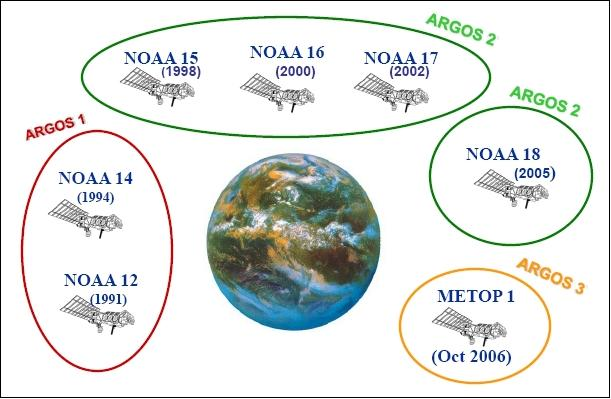
\includegraphics[width=\linewidth]{figures/argos_history.jpeg}
\caption{Three generations of Argos implementations on LEO S/C during the last two decades (image credit: Service Argos Inc.). Source: \url{https://directory.eoportal.org/web/eoportal/satellite-missions/a/argos-dcs}}
\label{fig:argos}
\end{figure}

%-----------------------------------
% GOES 
%-----------------------------------
\subsubsection{GOES Family}
\label{sssec:goes}


\ac{goes} is a joint \ac{noaa}/\ac{nasa} weather satellite series, where \ac{noaa} is responsible for funding, requirements and operation of the system in orbit, and \ac{nasa}, under contract fron \ac{noaa}, is responsable for spacecraft procurement, design, development of instruments and launch. \ac{noaa} owns and operates the satellites and provides the services to the user community.

Two meteorological satellites are placed in geostationary orbit. Each of these spacecraft views almost a third of the Earth's surface: one monitors North and South America and most of the Atlantic Ocean, the other North America and the Pacific Ocean basin. GOES-East is nominally positioned at 75\deg W longitude over the equator, while GOES-West is nominally positioned at 135\deg W longitude over the equator plane. The two spacecraft operate together to produce a full-face picture of the Earth, day and night. Coverage extends approximately from 20\deg W to 165\deg E longitude (see table \ref{tb:goes}).

Starting with GOES-I (GOES-8 on-orbit) each satellite carries two separate so-called second generation instruments, an imager and a sounder, providing simultaneous imaging and sounding capabilities. 

The \textbf{\ac{goes} Imager} is a multispectral imaging radiometer with one channel in the \ac{vis} and four channels in the \ac{ir} range , for operational meteorology and climatology (Table \ref{tb:goes_imager}). 


The \textbf{\ac{goes} Sounder}  is an infrared sounder for operational meteorology and climatology. Data products are: vertical temperature and moisture profiles, layer mean temperature and moisture, cloud height and amount, total precipitable water, surface temperatures, lifted index, gradient and wind derived from horizontal temperature and moisture fields.

The \ac{goes} satellites also carried aboard a \ac{sem} package to monitor "space weather"\footnote{\url{https://directory.eoportal.org/web/eoportal/satellite-missions/g/goes-2nd-generation}}\footnote{\url{https://directory.eoportal.org/web/eoportal/satellite-missions/g/goes-n-o-p}}.

\begin{table}
\center
\caption{\ac{goes} Family. Source: \url{https://directory.eoportal.org/web/eoportal/satellite-missions/g/goes-2nd-generation}}
\label{tb:goes}
\begin{tabularx}{\textwidth}{L{0.7}L{0.6}L{0.6}L{2.6}L{0.5}}
\toprule
Spacecraft & Launch & End & Comment & S/C Generation \\
\midrule 
ATS & Dec 1966 \newline May 1974 &  & \ac{ats} was a series of 6 weather \ac{geo} satellites 
with the purpose to test new technologies (spin stabilization, gravity gradient stabilization, demonstration of data collection from remote terminals, etc.) for communications and to investigate the geostationary orbit environment & Demo in \ac{geo} \\
\hline
SMS-1/2 \newline (SMS-A/B) & May 1974 \newline Feb 1975 & Jan 1981 & \ac{sms-1} was the first operational \ac{geo} weather satellite, located at 45\deg W. \ac{fd} images every 30 min & \\
\midrule
GOES-1/7 \newline  (GOES-A/H) & Oct 1975 \newline Feb 1987 & Mar 1985 \newline Apr 2012 & GOES-1 to -3 main instrument was \ac{vissr}.\newline GOES-4 was the first to measure a vertical profile of temperature and moisture with \ac{vas}. \newline GOES-7 was the sole geostationary spacecraft from 1989 to 1994 and the first spacescraft with a \hl{S\&RSAT} system flown. & 1st \\ 
\midrule
GOES-8/12 \newline (GOES-I/M) & Apr 1994 \newline & July 2001 &  After 10 years of service, GOES-8 was boosted into a higher orbit (\hl{350 km above GEO}). \newline GOES-9 was operational from 1995-1998 and from 2003-2007 was a backup for Japanese GMS-5. & \\
\midrule
GOES-13,14,15 \newline (GOES-N,0,P) & Apr 2010 \newline storage  \newline Dec 2011 & & GOES-13 is locates at 75\deg W (GOES East). \newline GOES-14 is located at 105\deg W (on orbit storage). \newline GOES-15 is located at 135\deg W  (GOES West) & 2nd \\
\midrule
GOES-R & Nov 2016 &  & First 3rd generaton with instruments \ac{abi} and \hl{SUVI,EXIS,GLM,SEISS,MAG} & 3rd \\
\midrule
GOES-S & Planned 2018 & & & \\
\bottomrule
\end{tabularx}
\end{table}





\begin{table}
\center
\caption{\ac{goes} Imager Instrument. Source:\url{https://directory.eoportal.org/web/eoportal/satellite-missions/g/goes-2nd-generation} and \url{https://directory.eoportal.org/web/eoportal/satellite-missions/g/goes-n-o-p}}
\label{tb:goes_imager}
\begin{tabularx}{\textwidth}{L{0.5}L{1}L{1}L{1}L{1.5}}
\toprule
Channel \newline Name & Channel \newline No & Spectral \newline Range [um] & Resolution \newline [km at nadir] & Measurment Objective \\
\midrule
VIS & 1 (GOES-I/M) \newline  1 (GOES-N/P) &  0.55 - 0.75 \newline 0.52 - 0.71 & 1 & Daytime cloud cover \\
\midrule
MWIR & 2 (GOES-I/J/K) \newline 2 (GOES-L/M) \newline 2 (GOES-N/P) & 3.80 - 4.00 \newline 3.80 - 4.00 \newline 3.73-4.07 & 4 & Nighttime clouds, fires, volcanoes\\
\midrule  
MWIR & 3 (GOES-I/J/K/L) \newline 3 (GOES-M) \newline 3  (GOES-N/P) &  6.50 - 7.00 \newline 13.0 - 13.7 \newline 5.80 - 7.30 & 8 & Water vapor \newline Cloud cover and height \\ 
\midrule 
TIR & 4 & 10.20 - 11.20 & 4 & Surface temperature and water vapor \\
\midrule
TIR & 5 (GOES (I/J/K/L) \newline 5 (GOES-M) \newline 5 (GOES-N/P) & 11.50 - 12.50 \newline 5.8 - 7.3 \newline 13.00 - 13.70 & 4  \newline (8 on GOES-N) & Surface temperature and water vapor \newline Water vapor \newline Cloud cover and cloud height \\
\bottomrule
\end{tabularx}
\end{table}

\begin{figure}
\centering
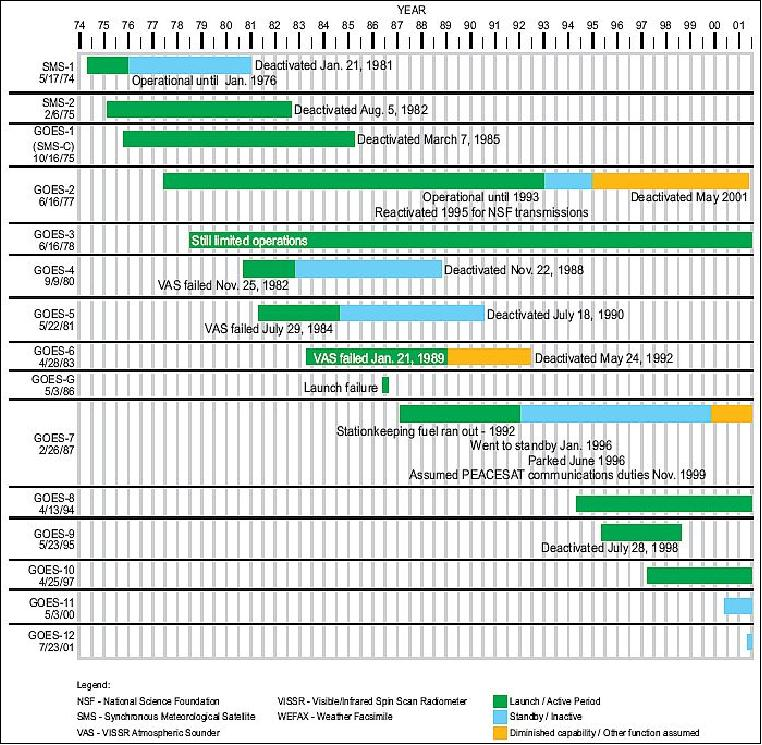
\includegraphics[width=\textwidth]{figures/GOES2_AutoB.jpeg}
\caption{Summary of GOES 1st and 2nd generation missions (image credit: NASA, NOAA). Source: \url{https://directory.eoportal.org/web/eoportal/satellite-missions/g/goes-2nd-generation}}
\label{fig:goes2nd}
\end{figure}

\begin{figure}
\centering
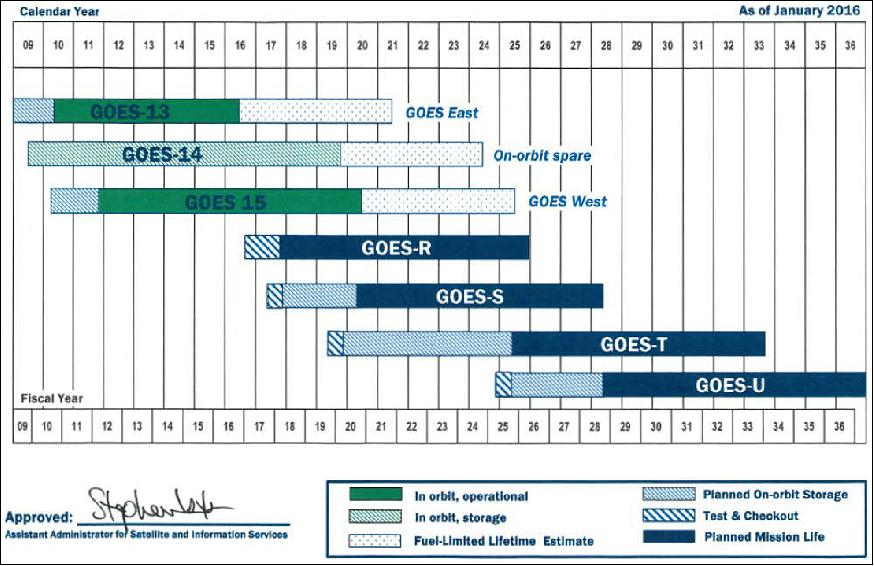
\includegraphics[width=\textwidth]{figures/GOES_NOP_Auto10.jpeg}
\caption{
Continuity of the GOES program as of January 2016 (image credit: NOAA). Source: \url{https://directory.eoportal.org/web/eoportal/satellite-missions/g/goes-n-o-p}}
\label{fig:goesnop}
\end{figure}

%-----------------------------------
% GOES-R 
%-----------------------------------
\paragraph{GOES-R}
\label{sssec:goesr}

\hl{todo - lots of differnt instruments} 
\url{https://directory.eoportal.org/web/eoportal/satellite-missions/g/goes-r}


%-----------------------------------
% POES 
%-----------------------------------
\subsubsection{POES Family}
\label{sssec:poes}



%-----------------------------------
% Copernicus 
%-----------------------------------
\subsection{Copernicus}
\label{ssec:copernicus}

Copernicus is the new name for the \ac{gmes} programme. 

This initiative is headed by the \ac{ec} in partnership with the \ac{esa}.

\ac{esa} coordinates the delivery of data from upwards of 30 satellites and the \ac{ec}, acting on behalf of the European Union, is responsible for the overall initiative, setting requirements and managing the services\footnote{\url{http://www.esa.int/Our_Activities/Observing_the_Earth/Copernicus/Overview3}}.

\ac{esa} is developing a new family of satellites, called Sentinels (section \ref{ssec:sentinels}) specifically for the operational needs of the Copernicus programme.

This programme is the European contribution to the worldwide \ac{geoss}.

The Copernicus Space Component comprises two types of satellite missions, ESA's families of dedicated Sentinels and missions from other space agencies, called Contributing Missions. A unified ground segment, through which the data are streamed and made freely available for Copernicus services, completes the Space Component.


% ------------------------------------------
% Introduction
% ------------------------------------------
\section{Satellites}
\label{sec:satellites}

\hl{optical, radar and altimetry}
\hl{geostationary, polar}
\hl{SAR}
\hl{multispectral}
\hl{sounder}

\subsection{FY-4}
\label{fy-4}

FY-4 is \ac{cma}'s second-generation three-axis stabilized, geostationary meteorological satellite series, under development by \ac{cast}. Two variants of spacecraft of the FY-4 (FenYun means "winds and clouds or storm" in Chinese) program are in planning, with one carrying optical sensors and the other carrying microwave sensors.

Compared to the current FY-2 geostationary meteorological satellite series, the performance of the FY-4 series has been considerably improved in terms of data amount, network transmission bandwidth, product type and quantity and archiving data and applications. The new generation FY-4 satellites are designed with an enhanced imagery scanning capability, desirable for monitoring small and medium scale weather systems. FY-4 is enabled with vertical atmospheric sounding and microwave detection capabilities to address 3D remote sensing at geostationary altitudes. The new FY-4 series is also enabled with solar observations for EUV (Extreme Ultraviolet) and X-ray monitoring, in a bid to enhance China's space weather watch and warning capability. 1)

Based on user requirements and technical feasibility, the missions of the FY-4 series include imagery, sounding, lightning mapping, and space environment monitoring. HRIT (High Rate Information Transmission), LRIT (Low Rate Information Transmission) data transmission, and DCP (Data Collection Platform) services are available for users. 2) 3) 4) 5)

In 2015, the Chinese government approved the NSIP (National Space Infrastructure Plan) covering also the meteorological program of LEO and GEO missions up to 2025. 6)


\begin{table}[h!]
\centering
\caption{The FY family. Source: \url{https://directory.eoportal.org/web/eoportal/satellite-missions/f/fy-4}}
\label{tb:fy4_vs_fy2}
\begin{tabularx}{\textwidth}{L{0.4}L{1.3}L{1.3}}
\toprule
Instrument & FY-4 & FY-2 \\ 
\midrule
Imaging &   \textbf{AGRI} (Advanced Geosynchronous Radiation Imager) (AGRI) \newline 
            14 channels \newline
            Spatial resolution: 0.5-4 km \newline
            \ac{fd} imaging: 15 min \newline 
            Rapid Scan: 2.5 min 
        &   \textbf{VISSR} (Visible and Infrared Spin-Scan Radiometer\newline
             5 channels \newline
            Spatial resolution: 1.25-5 km \newline
            \ac{fd} imaging: 30 min \newline
            Rapid Scan: 3-6 min \\
\midrule
Sounding & \textbf{GIIRS} (Geostationary Interferometric Infrared Sounder) \newline
            913 channels \newline
            Spectral resolution: 0.8 to 1.6 $cm^{-1}$ \newline
            Spatial resolution: 16 km 
        &  Not Applicable \\
\midrule
Lightning \newline 
Mapping &   \textbf{LMI} (Ligthning Mapping Imager) \newline   
            \hl{SSP} resolution: 7.8 km
        &  Not Applicable \\
\midrule
&   \textbf{SEP} (Space Environment Package) \newline
    High energy particles \newline
    Magnetic field: Solar X ray fluxes 
&   \textbf{SEM} (Space Environment Monitor) \newline
    High energy particles \\
\bottomrule
\end{tabularx}
\end{table}


\begin{figure}[h!]    
\centering
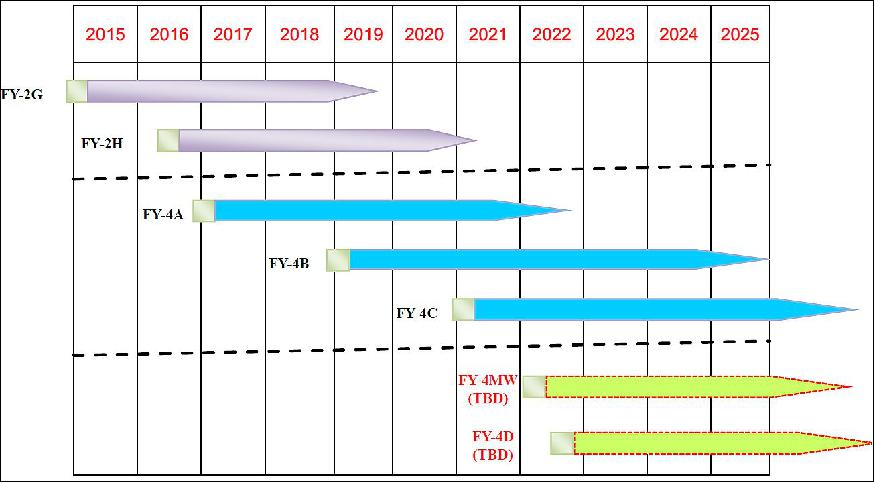
\includegraphics[width=\linewidth]{figures/FY4_Auto4.jpeg}
\caption{Overview of the GEO meteorological launch program of CMA for the next decade (image credit: CMA, source: \url{https://directory.eoportal.org/web/eoportal/satellite-missions/f/fy-4}}
\label{fig:fy4}
\end{figure}




\subsection{Proba-V}
\label{probaV}
Proba-V (V for Vegetation) is a ESA Miniature satellite (140 kg), launched in May 2013\footnote{\url{http://www.esa.int/Our_Activities/Space_Engineering_Technology/Proba_Missions/Overview2}}. 

It provides global coverage every two days, with latitudes 35-75\deg N and 35-56\deg S covered daily, and between 35\deg S and 35 \deg N  every 2 days. 
The Proba-V imager's continent-spanning 2250 km field of view collects light in the blue, red, near-infrared and mid-infrared wavebands, ideal for monitoring plant and forest growth as well as inland water bodies. The Vegetation instrument can distinguish between different land cover types and plant species, including crops, to reveal their health, as well as detect water bodies and vegetation burn scars.

The ESA Earth Watch Programme provides 1km data, which is complemented by a National Programme supplying products at 300m/600m resolution (available as ESA Third Party Mission)\footnote{\url{https://earth.esa.int/web/guest/missions/esa-operational-eo-missions/proba-v}}

The Proba-V image at 300 m resolution, acquired mid July 2016,takes a closer look at the South island of New Zealand (see Figure \ref{fig:nz_probaV}).

\begin{figure}[h!]    
\centering
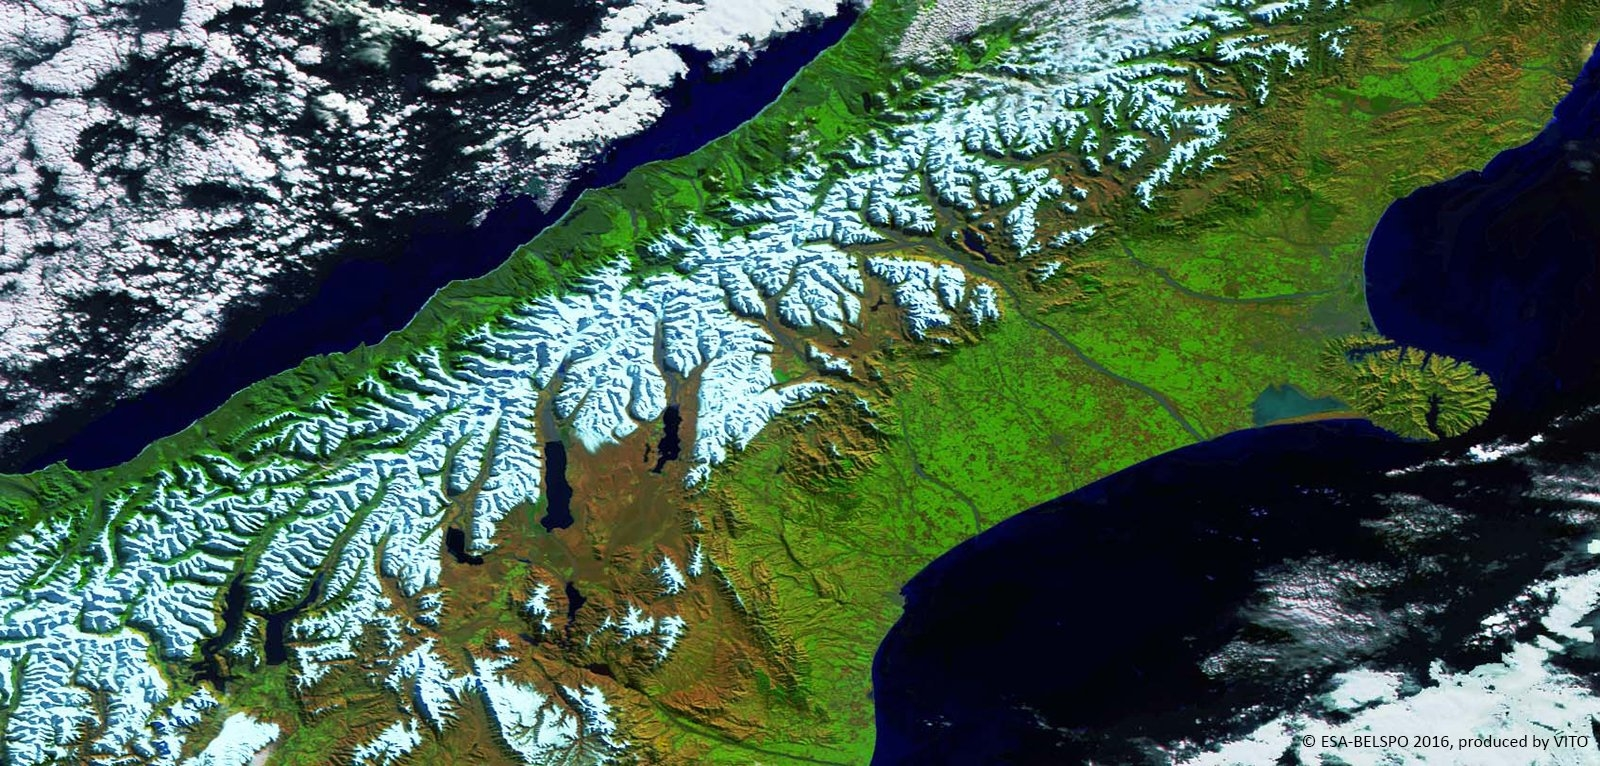
\includegraphics[width=\linewidth]{figures/New-Zealand_probaV.png}
\caption{South Island of New Zealand captured by Proba-V at 300 m resolution, mid July 2016
Source: \url{https://earth.esa.int/web/guest/missions/esa-operational-eo-missions/proba-v/image-of-the-week/-/article/new-zealand}}
\label{fig:nz_probaV}
\end{figure}

\subsection{SMOS}

ESA's \ac{smos} Earth Explorer mission is a radio telescope in orbit, but pointing back to Earth not space. It's \ac{miras} radiometer picks up faint microwave emissions from Earth's surface to map levels of land soil moisture and ocean salinity. These are the key geophysical parameters, soil moisture for hydrology studies and salinity for enhanced understanding of ocean circulation, both vital for climate change models.\footnote{\url{https://earth.esa.int/web/guest/missions/esa-operational-eo-missions/smos}}


\subsection{Sentinels}
\label{ssec:sentinels}

The Sentinels are a family of satellites developed specifically for the operational needs of the Copernicus programme (see section \ref{ssec:copernicus}). 

Each Sentinel mission is based on a constellation of two satellites to fulfil revisit and coverage requirements. 

These missions carry a range of technologies, such as radar and multi-spectral imaging instruments for land, ocean and atmospheric monitoring:

\begin{itemize}

\item \textbf{Sentinel-1} is a polar-orbiting, all-weather, day and night radar mission for land and ocean services. Sentinel-1A and -1B were launched respectively in April 2014 and April 2016. Both were taken into orbit on a Soyuz rocket from Europe's Spaceport in French Guiana.

\item \textbf{Sentinel-2} is a polar-orbiting multispectral mission delivering high-resolution optical images for land services, for example, imagery of vegetation, soil and water cover, inland waterways and coastal areas. Sentinel-2 can also deliver information for emergency services. Sentinel-2A was launched on 23 June 2015 and Sentinel-2B followed on 7 March 2017. 

\item \textbf{Sentinel-3} is a multi-instrument mission that provides high-accuracy optical, radar and altimetry data for marine and land services, for example, sea surface height, sea and land surface temperature, ocean colour and land colour. The mission will support ocean forecasting systems, as well as environmental and climate monitoring. Sentinel-3A was launched on 16 February 2016. 

\item \textbf{Sentinel-4} is devoted to atmospheric composition monitoring and will be embarked upon a \ac{mtg-s} satellite in geostationary orbit. 

\item \textbf{Sentinel-5} will also provide data for atmospheric composition monitoring but from a polar orbit, aboard a MetOp Second Generation satellite.

\item \textbf{Sentinel-5 Precursor} mission is being developed to reduce data gaps between Envisat, in particular the Sciamachy instrument, and the launch of Sentinel-5. 

\item \textbf{Sentinel-6} will carry a radar altimeter to measure global sea surface height, primarily for operational oceanography and for climate studies. 

\end{itemize}

\begin{figure}[h!]    
\centering
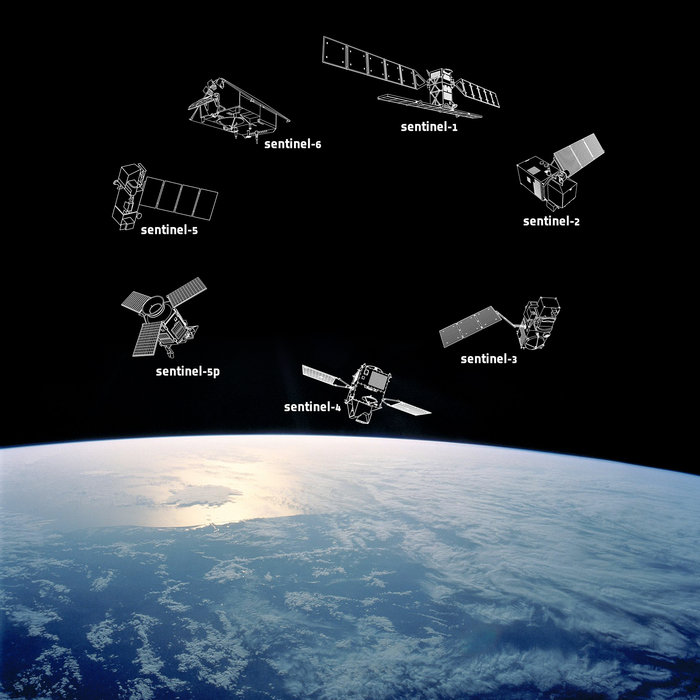
\includegraphics[width=0.5\linewidth]{figures/Sentinel_family_node_full_image_2.jpg}
\caption{The Sentinel family. Source: \url{http://www.esa.int/var/esa/storage/images/esa_multimedia/images/2014/04/sentinel_family/14493549-1-eng-GB/Sentinel_family_node_full_image_2.jpg}}
\label{fig:sentinels}
\end{figure}

\begin{table}[h!]
\centering
\caption{The Sentinel family.}
\label{tb:sentinels}
\begin{tabularx}{\textwidth}{C{0.2}C{0.5}L{0.8}L{2.5}}
\toprule
Sentinel & Orbit & Period & Description of Mission \\ 
\midrule
1 & Polar & 1-A: Apr 2014\newline1-B: Apr 2016 & All weather, day and night radar \\
\midrule
2 & Polar & 2-A: Jun 2015\newline2-B: Mar 2017 & Hi-res optical (multispectral) for land; Emergency services \\
\midrule
3 &       & 3-A: Feb 2016 & Multi-instrument: optical, radar and altimetry; Land and marine services: SSH, SST, LST, colour \\
\midrule
4 & Geo &  & Atmospheric composition, aboard MTG \\
\midrule
5 & Polar &  & Atmospheric composition, aboard Metop \\
\midrule
5P & Polar & & Reduce data gaps between Envisat (Sciamachy instrument) and S-5 \\
\midrule
6 & & & radar altimeter to measure global SSH \\                                           
\bottomrule
\end{tabularx}
\end{table}

% ------------------------------------------
% End Matter
% ------------------------------------------
\clearpage
% \addcontentsline{toc}{part}{References}
% \renewcommand{\bibname}{References}
% \bibliographystyle{styles/agufull}
% \bibliography{library}
% \label{sec:references}

\printacronyms
\end{document}
% ------------------ End of Document --------------------%
